\chapter{Relativité avec gravitation : fondements}

    \section{Principe d'équivalence}
    
        Quelle que soit la relativité (galiléenne ou einsteinienne), rien n'explique pourquoi les référentiels inertiels sont tels que observés. L'observation montre que le référentiel lié au soleil avec des axes pointants vers les étoiles "fixes" est un excellent référentiel inertiel. Cependant, si l'on prend du recul, ce référentiel n'est pas mieux qu'un autre. Qu'est-ce qui détermine les référentiels inertiels alors ?\\
            
        Voici une petite expérience de pensée qui permet de mieux se rendre compte du problème. Imaginons être dans le vide, sans lumière, sans son, sans aucun repère. Juste en face de nous, flottent deux boules de liquide, du whisky par exemple. Celle de gauche est sphérique et celle de droite est ellipsoïdale. On peut alors dire que la boule de gauche est immobile dans un référentiel $\R$ et que celle de droite est en rotation par rapport à $\R$. Mais qu'est-ce qui détermine ce référentiel à ce point dans l'espace ?\\
        
        Le physicien E. Mach avait déjà mis en évidence la relation entre les référentiels inertiels et les étoiles "fixes", c'est-à-dire la distribution de masse dans l'univers. Il a alors tenté d'appliquer ce principe en mesurant une potentielle différence de force d'inertie entre le plan de la galaxie et le plan transverse. Mais en réalité, il n'existe pas d'anisotropie de l'inertie, cependant l'idée de Mach est conceptuellement correcte.\\
        
        Ce problème est en fait lié au premier problème dont nous avons déjà parlé : mettre en place en théorie relativiste de la gravitation.
    
        \subsection{Énoncé du principe}
        
            Commençons par discuter le principe d'équivalence dans sa version la plus traditionnelle.
            
            \begin{prin}[d'équivalence, première formulation]
            \begin{leftbar}
                La masse gravitationnelle est égale à la masse inertielle.
            \end{leftbar}
            \end{prin}
            
            Dans sa seconde loi, Newton nous dit que pour un corps de masse $m_i$, la force résultante qui s'exerce sur ce corps est reliée à son accélération par
            \begin{equation}
                \vv{F} = m_i\vv{a}.
            \end{equation}
            
            D'un autre coté, la loi de la gravitation universelle de Newton dit que le champ de gravitation créé par un corps de masse $m_g$ situé en $O$ est donné par
            \begin{equation}
                \vv{g}(M) = -\frac{m_g G}{\abs{\vv{OM}}^3}\vv{OM}.
            \end{equation}
            
            Mais rien ne garanti que les paramètres $m_i$ et $m_g$ soient identiques. A priori, ce sont deux propriétés distinctes d'un corps qui apparaissent dans deux phénomènes différents. La masse apparaissant dans la seconde loi de Newton est appellée \textit{masse inertielle} et la masse apparaissant dans la loi de la gravitation universelle est appelée \textit{masse gravitationnelle} (c'est la "charge gravitationnelle").\\
            
            Si $m_i\neq m_g$, il y aurait des conséquences mesurables. Prenons l'exemple d'un pendule : dans un régime de petites oscillations, la période est donnée par
            \begin{equation}
                T = 2\pi\sqrt{\frac{m_iL}{m_g g}}
            \end{equation}
            où $L$ est la longueur du pendule. L'expérience d'Eötvos permet également de calculer le rapport $\nicefrac{m_i}{m_g}$ avec une très grande précision. Celle-ci fonctionne comme suit : on suspend deux corps différents à chaque extrémité d'une barre qui est elle-même suspendue à un support fixe. Alors, si les corps ont des masses de rapport $\nicefrac{m_{i}}{m_g}$ différents, les forces d'inerties dûes à la rotation de la Terre devraient entraîner une torsion sur le fil. Cette expérience a pu montrer que $m_i = m_g$ avec une très grande précision.\\
            
            En 1907, Einstein va prendre cette idée très au sérieux et partir de cette hypothèse pour construire une théorie relativiste de la gravitation qui sera aussi automatiquement une théorie de l'inertie.\\
            
            Observons une conséquence de cette hypothèse. Supposons que l'on ait le bilan de forces suivant dans un référentiel inertiel $\R_1$:
            \begin{equation}
                m_i\vv{a}_{\R_1} = m_g\vv{g} + \vv{F}.
            \end{equation}
            Dans un référentiel $\R'$, il y a des forces d'entraînement et des forces d'inertie qui apparaissent:
            \begin{equation}
                m_i\vv{a}_{\R_2} = m_g\vv{g} -m_i\vv{a}_e-m_i\vv{a}_i + \vv{F}.
            \end{equation}
            En regroupant les termes et en utilisant le principe d'équivalence, nous pouvons interpréter le référentiel $\R_2$ comme étant lui-même inertiel mais dont le champ de gravitation est maintenant $\vv{g}'$.
            \begin{equation}
                m\vv{a}_{\R_2} = m(\underbrace{\vv{g} -\vv{a}_e-\vv{a}_i}_{\vv{g}'}) + \vv{F}
            \end{equation}
            Il n'est donc pas possible, si $m_i=m_g$, de distinguer les effets d'une force gravitationnelle et d'une force d'inertie : c'est le principe d'équivalence entre gravitation et inertie. Passons maintenant à une formulation plus précise du principe d'équivalence.
            
            \begin{prin}[d'équivalence, deuxième formulation]
            \begin{leftbar}
                Dans une région suffisamment petite de l'espace-temps, il est toujours possible de choisir un référentiel dans lequel le champ de gravitation s'annule.
            \end{leftbar}
            \end{prin}
        
            Cette formulation du principe est beaucoup plus géométrique, on verra dans la suite que l'on peut considérer l'espace-temps comme un espace courbe. Le principe d'équivalence stipule qu'il est toujours possible de trouver un système de coordonnées tel que l'espace-temps est localement assimilable à un plan, c'est-à-dire à l'espace-temps plat de Minkowski. Cette idée permettra de relier le champ de gravitation aux propriétés géométriques de l'espace-temps.
        
        \subsection{Applications simples du principe d'équivalence}
        
            \subsubsection{Déviation d'un rayon lumineux par un champ de gravitation}
            
                Si un objet peut être vu comme allant en ligne droite dans un référentiel, un changement de référentiel (rotation) permet de le voir se déplacer suivant une trajectoire courbe. En utilisant le principe d'équivalence, ceci implique que le champ de gravitation peut dévier les rayons lumineux.\\
                
                Imaginons une étoile située derrière le soleil du point de vue de la Terre. On peut montrer en mécanique classique que n'importe quel corps allant à une vitesse $\vv{v} = \vv{c}$ subirait un angle de déviation
                \begin{equation}
                    \Delta\varphi = 2\frac{GM_\odot}{ac^2}
                \end{equation}
                où $a$ est le paramètre d'impact. Cette formule peut être obtenue en quasi-totalité par analyse dimensionnelle mais le facteur 2 lui provient des lois de Newton. En voyant la lumière comme composée de corps massiques on obtient alors que les rayons lumineux provenant d'une étoile derrière le soleil seraient déviés d'un angle $\Delta\varphi$.\\
                
                Les mêmes calculs dans la théorie d'Einstein permettent de trouver un angle de déviation
                \begin{equation}
                    \Delta\varphi = 4\frac{GM_\odot}{ac^2}
                \end{equation}
                au premier ordre. Le facteur $4$ est bien différent de celui prédit par Newton.\\
                
                En 1919, A. Eddington a organisé une expédition lors d'une éclipse solaire totale pour mesurer l'angle de déviation des rayons parvenant d'une étoile par le soleil. Les résultats sont précisément ceux prédit par le théorie d'Einstein. C'est une des premières validations expérimentales de la relativité générale.
            
                \begin{figure}[H]
                \centering
                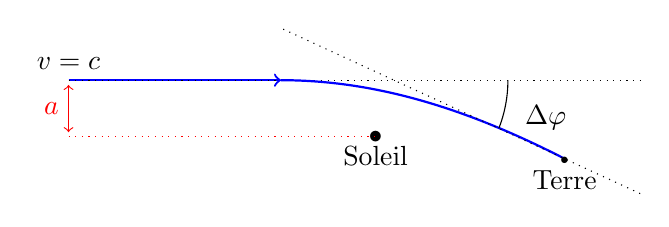
\begin{tikzpicture}[scale = 6]
                    \draw[->, thick, blue] (-0.45, 0) node[above, black]{$\Vec{v} = \Vec{c}$} -- (0,0);
                    \draw[dotted] (-0.45, 0) -- (0.76,0);
                    \draw[domain = 0:0.6, thick, smooth, blue] plot(\x, {-sqrt(1 + \x*\x) + 1});
                    \draw (0.48, 0) arc (0: -21.3 : 0.28);
                    \draw[dotted] (0.76, -0.24) -- (0,0.11);
                    \draw (0.56, -0.08) node{$\Delta \varphi$};
                    \draw (0.6, -0.17) node[scale = 0.6]{$\bullet$} node[below]{Terre};
                    \draw (0.2, -0.12) node{$\bullet$} node[below]{Soleil};
                    \draw[<->, red] (-0.45, -0.01) -- (-0.45, -0.11) node[midway, left]{$a$};
                    \draw[dotted, red] (-0.45, -0.12) -- (0.2, -0.12);
                    \end{tikzpicture}
                \caption{Déviation d'un rayon lumineux par le soleil}
                \end{figure}
            
            \subsubsection{Distorsion du temps par un champ de gravitation}
            
                On regarde les phénomènes sur une échelle de distance $h$. Quelle est la variation typique d'un potentiel gravitationnel sur échelle $h$ ? Considérons deux observateurs $A$ et $B$ au voisinage d'un astre de masse $M$ tels que $z_B-z_A\equiv h>0$ où $z$ dénote l'altitude. Le potentiel newtonnien généré par l'astre est
                \begin{equation}
                    V(z) = \frac{GM}{z}
                \end{equation}
                Ainsi, la différence de potentiel entre observée entre les points $A$ et $B$ est
                \begin{equation}
                    V(z_B)-V(z_A) = GM\left( \frac{1}{z_A+h} -\frac{1}{z_A}\right)=-\frac{GM}{z^2_A}h+\order{H^2} = g(z_A)h +\order{h^2}
                \end{equation}
                où $g$ est e champ de gravitation local. Nous obtenons $\delta V\sim gh$.
                \begin{definition}
                    On définit le \textit{paramètre de relativité} comme le rapport
                    \begin{equation}
                        \Xi = \frac{\abs{V}}{c^2}.
                    \end{equation}
                    où $\abs{V}$ est l'échelle de potentiel considérée.
                \end{definition}
                \begin{definition}
                La \textit{limite de champ faible} exprime le fait que l'approximation newtonienne et bonne, c'est-à-dire que
                \begin{align}
                    \Xi\ll1.
                \end{align}
                \end{definition}
                Dans notre cas, $\frac{gh}{c^2}\ll1$.\\
            
                On considère un champ de gravitation constant $\vv{g}=-g\vv{u}_z$ dans le référentiel $\R$ et deux observateurs : $E$ (émetteur) situé à un hauteur $z_E$ et $R$ (récepteur) situé à une hauteur $z_R = z_E+h$. Supposons que l'émetteur émette un signal, de période $(\delta t)_E = t_2^E-t_1^E$. Le signal est reçu par un le récepteur aux temps $t_1^R,t_2^R$, il observe donc une période $(\delta t)_R = t_2^R-t_1^R$. En vertu du principe d'équivalence, ce champ de gravitation est équivalent à un observateur uniformément accéléré dans la direction $\vv{u}_z$. De ce point de vue, $E$ et $R$ ont les positions
                \begin{align}
                    z_E(t) &=  \frac{1}{2}gt^2 \\
                    z_R(t) &= h  \frac{1}{2}gt^2
                \end{align}
                Si $z_1(t)$ et $z_2(t)$ sont les trajectoires des pulses alors
                \begin{align}
                    z_1(t) &= c(t-t^E_1) \\
                    z_2(t) &= c(t-t_2^E)
                \end{align}
                
                % schéma Eliott
                
                Calculons les temps de réception. Par définition, on doit avoir
                \begin{subequations}
                \begin{empheq}[left=\empheqlbrace]{align}
                    z_1(t_1^R-t^E_1) &= z_R(t_1^R) \\
                    z_2(t_2^R) &= z_R(t_2^R)
                \end{empheq}
                \end{subequations}
                autrement dit,
                \begin{subequations}
                \begin{empheq}[left=\empheqlbrace]{align}
                    ct_1^R &= h-\frac{1}{2}g(t_1^R)^2 \\
                    c(t_2^R-t_2^E) &= h-\frac{1}{2}g(t_2^R)^2
                \end{empheq}
                \end{subequations}
                Si l'on considère le cas $\dot{z}_1(t),\dot{z}_2(t)\ll c$ et $gt\ll c$ (limite de champ faible), on peut alors développer au premier ordre après avoir soustrait les deux équations précédentes.
                \begin{equation}
                    c\left( (\delta t)_R-(\delta t)_E \right) = \frac{1}{2}g\left( (t_2^R)^2-(t_1^R)^2 \right) \approx \frac{gh}{c}(\delta t)_R
                \end{equation}
                On trouve alors que
                \begin{align}
                    (\delta t)_R-(\delta t)_E &=  \frac{gh}{c^2}(\delta t)_R \\
                    \Leftrightarrow\quad (\delta t)_E &= \left( 1-\frac{gh}{c^2} \right)(\delta t)_R  \\
                    \Leftrightarrow\quad \nu_R &= \left( 1-\frac{gh}{c^2} \right)\nu_E
                \end{align}
                où $\nu_E = \frac{1}{(\delta t)_E}$, $\nu_R = \frac{1}{(\delta t)_R}$ sont respectivement les fréquences d'émission et de réception.\\
                
                En posant $\nu\approx \nu_1 \approx \nu_2$ (la différence entre $\nu_1$ et $\nu_2$ est très petite),
                \begin{equation}
                    \frac{\Delta\nu}{\nu} = -\frac{gh}{c^2}
                \end{equation}
                
                Voici un second raisonnement : lorsque l'observateur accéléré arrive au niveau de $R$, il coïncide avec un observateur de vitesse constante $v = g(\delta t)_E = \frac{gh}{c}$. Par effet Doppler, ce dernier observe une plus petite fréquence que celle à laquelle $E$ a émit le signal.
                \begin{equation}
                    \frac{\nu_E}{\nu_R} = \sqrt{\frac{1+\frac{gh}{c^2}}{1-\frac{gh}{c^2}}}\approx 1+\frac{gh}{c^2}.
                \end{equation}
                ce qui correspond au résultat que nous avions trouver en premier lieu. La fréquence observée est donc plus petite que le fréquence émise.\\
                Pour un champ non-uniforme, cette formule se généralise comme
                \begin{equation}
                    \frac{\Delta\nu}{\nu} = -\frac{\Delta\phi}{c^2}
                \end{equation}
                où $\varphi$ est le potentiel du champ $\vv{g}$, c'est-à-dire le champ tel que $\vv{g} = -\vv{\nabla}\varphi$.
                
                \begin{exmp}
                    Pour un rayon lumineux en provenance du soleil, $\varphi=-\frac{GM_\odot}{r}$ et donc
                    \begin{equation}
                        \Delta\varphi = -\frac{GM_\odot}{r_{\odot-\oplus}} + \frac{GM_\odot}{R_\odot}\approx\frac{GM_\odot}{R_\odot}.
                    \end{equation}
                    Ceci donne
                    \begin{equation}
                        \frac{\Delta\nu}{\nu} \approx - \frac{GM_\odot}{R_\odot c^2} = -\varepsilon_\odot \sim 10^{-6}.
                    \end{equation}
                    Il y a donc un décalage vers le rouge lorsque les rayons remontent le champ de gravitation. Cet effet est observable pour les raies spectrales.
                \end{exmp}
                
                On voit le temps des satellites en orbite autour de la Terre dilaté par effet cinématique (relativité restreinte) mais il y a aussi un effet inverse dû au champ de gravitation terrestre. On verra qu'il existe une orbite où ces effets se compensent.
    
        \subsection{Principe de covariance générale}
        
            Le principe d'équivalence dit que, localement dans l'espace-temps, les effets du champ de gravitation peuvent êtres annulé par un choix de référentiel approprié (référentiel localement inertiel). Pour connaître les lois de la physique en présence de gravitation dans un référentiel quelconque $\R$, il suffit donc faire un changement de référentiel à partir d'un référentiel localement inertiel (où les lois des la physique sont déjà connues mais sans gravitation) à $\R$. Donc, le principe d'équivalence permet de déduire les effets du champ de gravitation lorsque l'on connaît les lois de la physique en l'absence de gravitation, c'est un \textit{principe de covariance} et non un \textit{principe de symétrie} (ou \textit{principe d'invariance}).\\
            
            En particulier, ce principe est de nature fondamentalement différente du principe de relativité einsteinienne qui est un principe d'invariance. Ce dernier dit que les lois de la physique restent les mêmes (invariantes) sous les transformations du groupe de Poincaré. Ceci "contraint" la physique à s'écrire en terme de vecteurs (au sens de Poincaré), pas le principe d'équivalence.\\
            
            Néanmoins, les équations du champ de gravitation devront être décrites d'une manière générale dans tout les référentiels possibles, puisque l'effet des changements de référentiels n'est rien d'autre qu'un champ de gravitation. C'est le \textit{principe de covariance générale}. Il faut écrire les lois de la physique dans tout les référentiels. C'est une autre manière de reformuler le principe d'équivalence.
            
            \begin{prin}[de covariance générale]
            \begin{leftbar}
            Les lois de la physique doivent êtres écrites sous une forme qui ne fait référence à aucun référentiel.
            \end{leftbar}
            \end{prin}
            
            Le principe qui sous-tend la notion de covariance générale est qu'il n'existe a priori aucune coordonnée. Ces dernières sont seulement des artifices mathématiques utilisés pour décrire la nature et ne devraient donc jouer aucun rôle dans l'expression des lois de la physique. C'est une redondance et pas une symétrie, comme pour les transformations de jauge (ce qu'on appelle symétrie de jauge n'est en fait pas une symétrie).
    
    \section{Changement de référentiels et variétés}
    
        \subsection{Espaces courbes}
        
            En mécanique classique, la distance entre deux points est absolue. Ceci rend, entre autre, la notion de solide possible (ensemble de point à distance fixe). Mais en relativité restreinte ce n'est plus le cas. \\
            
            Notons $\M$ l'espace-temps. Quelle que soit sa nature, il doit être possible de "mettre" un système de coordonnées sur cet espace. L'espace-temps doit donc en quelque sorte être assimilable à $\mathbb{R}^4$. Rien ne dit qu'il doit exister une bijection de l'espace-temps de $\M$ dans $\mathbb{R}^4$ mais on doit en tout cas pouvoir couvrir $\M$ de domaines qui sont en bijection avec $\mathbb{R}^4$. C'est ici qu'intervient la notion de \textit{variété}.\\
            
            On commence par définir les fonctions qui font l'intermédiaire entre un ensemble quelconque (ici $\M$) et $\mathbb{R}^n$.
            \begin{definition}
                Une \textit{carte locale} $(U,\varphi)$ de dimension $n$ pour un ensemble $\M$ est une bijection
                \begin{equation}
                    \varphi:U\to\varphi(U) \subset\mathbb{R}^n
                \end{equation}
                où $U$ est un sous-ensemble de $\M$ appelé \textit{domaine de carte} et $\varphi(U)$ un ouvert de $\mathbb{R}^n$. La fonction $\varphi$ est appellée \textit{application de coordonnées}.
            \end{definition}
            
            Ce nom se justifie par le fait que notre fonction $\varphi$ est entièrement déterminée par ses coordonnées telles que $\varphi = (x^1, x^2, \ldots, x^n)$ où $x^i: U \to \mathbb{R}$ quel que soit $i$. Pour pouvoir couvrir tout l'espace-temps, nous avons besoin d'un ensemble de cartes dont les domaines recouvrent $\M$.
            
            \begin{definition}
                Un \textit{atlas différentiable} $\A$ de dimension $n$ pour un ensemble $\M$ est une collection 
                \begin{equation}
                    \A = \left\{ (U_i,\varphi_i)~|~i\in I \right\}
                \end{equation}
                de cartes locales de dimension $n$ pour $\M$ telle que
                \begin{enumerate}[label=\textit{(\roman*)}]
                    \item $\bigcup_{i\in I} U_i = \M$
                    \item si $U_i\cap U_j \neq \varnothing$ alors $\varphi_i(U_i\cap U_j)$ est un ouvert de $\Rm$ et les cartes $(U_i,\varphi_i)$ et $(U_j,\varphi_j)$ sont \textit{compatibles}, c'est-à-dire que l'application de changement de carte
                        \begin{equation}
                            \varphi_j\circ\varphi_i^{-1}:\varphi_i(U_i\cap U_j)\subset\Rm\to\varphi_j(U_i\cap U_j)\subset\Rm
                        \end{equation}
                        est différentiable (de classe $C^\infty$).
                \end{enumerate}
            \end{definition}
            
            Notons que nous travaillerons uniquement avec des applications différentiables. Pourquoi ne pas imposer directement que les applications de coordonnées soient différentiables ? A priori, $\M$ est juste un ensemble et ne comporte aucune structure supplémentaire, cette notion n'aurait donc pas de sens. De plus, nous verrons qu'un changement de carte correspond à un changement de référentiel. Les changements de carte doivent donc être différentiables afin de pouvoir écrire les lois de la physique (EDP) dans tous les référentiels. Ceci justifie l'utilisation de variétés dites "différentiables", et pas d'un autre type de variété.
            
            \begin{rmk}
                La condition de changement de carte différentiable permet en fait plus que cela. Lorsqu'on a une application entre deux variétés, on peut définir ce que différentiable signifie pour celle-ci. Pour que cette notion ne dépende pas des cartes choisies, il faut que les changement de carte soient eux aussi différentiables.
            \end{rmk}
            
            La prochaine définition demande de connaître plusieurs notions mathématiques que nous ne traiterons pas en détail dans ces notes.
            
            \begin{definition}
                Une \textit{variété différentiable} $(\M,\A)$ de dimension $n$ est un ensemble $\M$ munit d'un atlas différentiable de dimension $n$ tel que la topologie canonique associée soit séparée au sens de Hausdorff et à base dénombrable.
            \end{definition}
            
            Revenons sur les notions impliquées dans cette définition. Il possible de montrer qu'un ensemble de domaines de carte forme une topologie, on l'appelle \textit{topologie canonique}. On veut que cette topologie soit \textit{séparée au sens de Hausdorff}. Cela signifie que si l'on prend deux points $a, b \in \M$, il doit exister deux ouverts disjoints $U$ et $V$ tels que $a \in U$ et $b \in V$. Cela permet d'éviter le "dédoublement" de points. Pour finir, la topologie canonique doit aussi être \textit{à base dénombrable}, c'est-à-dire qu'il doit exister un ensemble dénombrable d'ouverts tels que n'importe quel autre ouvert peut s'exprimer comme une union (au plus dénombrable) d'ouverts de cet ensemble. Cette condition assure une certaine cohérence entre la dimension de la variété et l'ensemble en question. Sans cela, il serait, par exemple, possible de munir l'ensemble $\mathbb{R}^2$ d'un atlas de sorte à obtenir une variété différentiable de dimension $1$.
            
            \begin{rmk}
                Pour être rigoureux, on distingue la notion de structure différentiable et de variété différentiable. Une structure différentiable est une classe d'équivalence d'atlas différentiables. On dit que deux atlas sont équivalents si toutes leurs cartes sont compatibles, c'est-à-dire si l'union des deux atlas forme toujours un atlas différentiable. Notons que la donnée d'un atlas suffit à définir une classe d'équivalence. On définit alors une variété différentiable comme étant un ensemble munit d'une structure différentiable et dont la topologie canonique respecte les propriétés énoncées ci-dessus. Si l'on a une application $a$ entre deux variétés, on dit que $a$ est un homéomorphisme (notion d'équivalence pour les topologies) si $a$ est bijective et bicontinue. Les deux variétés sont alors homéomorphes. Si en plus $a$ est bidifférentiable, c'est un difféomorphisme et les variétés sont difféomorphes (notion d'équivalence pour les variétés différentiables). Si deux variétés sont difféomorphes elles sont aussi homéomorphes mais pas le contraire. Ceci permet au même ensemble d'avoir la même topologie canonique mais des structures différentiables non-difféomorphes. Par exemple, il a été montré (Milnor, 1964) que la sphère $S^n$ munit de la topologie induite par la topologie usuelle de $\mathbb{R}^{n+1}$ possède 28 structures de variétés différentiables non-difféomorphes pour $n=7$, une seule pour $n<7$ et un nombre qui croit rapidment pour $n>7$.
            \end{rmk}
            
            \begin{rmk}
                 Nous verrons dans l'on peut définir la notion de différentiabilité  pour une application entre deux variétés. On peut alors montrer que le fait d'imposer que les changements de carte soient différentiables implique que les carte sont aussi différentiables. Une variéte est donc localement difféomorphe à $\mathbb{R}^n$.
            \end{rmk}
            
            
            \begin{rmk}
            	Même si nous le ferons parfois pour définir certaines variétés (e.g. la sphère), il n'est pas nécessaire de voir une variété comme un espace "plongé" dans un espace plus grand. Une variété a une existence individuelle. Le terme "plongement" correspond à un concept bien précis en géométrie différentielle, nous désignons ici l'idée intuituve. On peut cependant montrer que toute variété de dimension $n$ peut être vue comme plongée dans $\mathbb{R}^{2n}$ (version forte du théorème de plongement de Whitney) mais dans le cas de la relativité générale, on considère que l'espace-temps à quatre dimension qui n'est pas plongé dans un espace de dimension supérieure.
            \end{rmk}
            
            \begin{prin}
            \begin{leftbar}
            	L'espace-temps, c'est-à-dire la collection de tout les évènements, est la donnée d'un couple $(\M,g)$ où $\M$ est une variété différentiable et $g$ est une métrique Lorentzienne sur $\M$.
            \end{leftbar}
            \end{prin}
            
            \begin{rmk}
            	La notion de tenseur métrique sera définie dans le chapitre suivant.
            \end{rmk}
            
            Dans ce cas, quel que soit $P\in\M$ un évènement, on a alors un domaine de carte $U$ avec $P\in U$ et une application de coordonnées
            
            \begin{equation}\label{eq:coordloc}
            x:\left(
            \begin{array}{ccc}
                U & \longrightarrow & x(U) \subset \mathbb{R}^4  \\
                P & \longmapsto & x(P) = (x^0(P), x^1(P) , x^2(P), x^3(P))
            \end{array}
            \right).
            \end{equation}
            
            \begin{definition}
                Si $x$ est une carte locale en $P\in\M$, alors on appelle \textit{coordonnées locales} du point $P$ les applications $x^\mu$ telles que \ref{eq:coordloc}.
            \end{definition}
            
            On utilise la notation $(x^\mu(P)) \equiv (x^0(P),x^1(P),x^2(P),x^3(P))$. De manière générale, lorsque que le contexte est clair, on ne note pas la dépendance en le point de l'espace-temps. Par exemple, $g_{\mu\nu}(P)\equiv g_{\mu\nu}$. Gardons bien à l'esprit que les coordonnées locales $x^\mu$ sont des applications et que les $x^\mu(P)$ sont des nombres réels. 
            
            \begin{definition}
                On dit que le système de coordonnées $z$ est \textit{localement plat} en $P$ si $(z,U)$ est une carte locale telle que $P\in U$ et 
                \begin{subequations}\label{locin}
                \begin{empheq}[left=\empheqlbrace]{align}
                    g_{\mu\nu}(P) &= \eta_{\mu\nu}\\
                    \p_\alpha g_{\mu\nu}(P) &= 0
                \end{empheq}
                \end{subequations}
                On note l'application de coordonnée $z_P$.
            \end{definition}
            
            Si $z_P$ est un système de coordonnées localement plat en $P$, et $Q\in U$ alors $z_P^\alpha(Q)$ sont les coordonnées de $Q$ dans le système de coordonnées localement inertiel en $P$.\\
            
            Nous avons vu précédemment que référentiel et système de coordonnées sont des notions équivalentes. Un changement de référentiel n'est donc rien d'autre qu'un changement de carte. Soient deux applications de coordonnées (deux système de coordonnées) $x^\mu$ et $x'^\mu$ au point $P\in\M$, alors on peut alors exprimer les coordonnées $x'^\mu(P)$ en fonction des coordonnées $x^\mu(P)$.
            \begin{equation}\label{eq:chgtref}
                x'^\mu(P) = (x'\circ x^{-1})(x^\mu(P))
            \end{equation}
            
            \begin{definition}
                Une \textit{ligne d'univers} est une courbe différentiable dans la variété, c'est-à-dire une application
                \begin{equation}
                    \gamma : I\subset\mathbb{R} \to \M.
                \end{equation}
            \end{definition}
            On peut directement obtenir une courbe dans $\mathbb{R}^4$ à partir de celle dans $\mathcal{M}$.
            \begin{equation}
                x^\mu(\lambda)\equiv(x\circ\gamma)(\lambda)
            \end{equation}
            Nous voudrions exprimer cette courbe en fonction du temps propre mais cette notion n'est pas encore claire dans ce formalisme.\\
            
            Soit $P\in\M$ un évènement et $z^\alpha_P$ des coordonnées localement inertielles en $P$. L'existence d'un tel système de coordonnées est garantie par le principe d'équivalence. Par définition, le temps propre doit satisfaire
            \begin{equation}
                d\tau^2 = -\eta_{\alpha\beta}dz^\alpha_Pdz^\beta_P
            \end{equation}
            Dans un référentiel quelconque de coordonnées $x$, cette relation devient
            \begin{equation}\label{eq:met}
                d\tau^2 = -\eta_{\alpha\beta}\frac{\p z^\alpha_P}{\p x^\mu}\frac{\p z^\beta_P}{\p x^\nu}~dx^\mu dx^\nu
            \end{equation}
            où l'on a utilisé $\ref{eq:chgtref}$. On obtient une expression de $\eta_{\mu\nu}$ généralisée (aux référentiels non-localement inertiels). Même si cela peut paraître claire, nous définirons mieux les objets du type $dz^\alpha_P$ dans le suite, cela justifiera cette loi de transformation.
            
            \begin{definition}
                Si $z$ est un système de coordonnées localement inertiel en $P$ et $x$ un autre système de coordonnée en $P$, on définit le \textit{tenseur métrique} comme
                \begin{equation}
                    g_{\mu\nu}(P)~\hat{=}~\eta_{\alpha\beta}\frac{\p z^\alpha_P}{ \p x^\mu}\frac{\p z^\beta_P}{\p x^\nu}
                \end{equation}
            \end{definition}
            Notons bien que le tenseur métrique dépend du point de l'espace-temps en lequel il est considéré.\\
            La relation \ref{eq:met} devient
            \begin{equation}
                d\tau^2 = -g_{\mu\nu}~dx^\mu dx^\nu.
            \end{equation}
            
            \begin{prop}\begin{leftbar}
                Le tenseur métrique satisfait les propriétés suivantes.
                \begin{enumerate}[label = \textit{\roman*)}]
                    \item symétrie : $g_{\mu\nu}=g_{\nu\mu}$
                    \item métrique : $g_{\mu\nu}$ définit un produit scalaire qui a la même signature que $\eta$
                    \item si $g'_{\mu\nu}$ est le tenseur métrique dans les coordonnées $x'(x)$ alors
                    \begin{equation}
                        g'_{\mu\nu} = \frac{\p x^\rho}{\p x'^\mu}\frac{\p x^\kappa}{\p x'^\nu}~g_{\rho\kappa}.
                    \end{equation}
                \end{enumerate}
            \end{leftbar}\end{prop}
            
            \begin{proof}
                \begin{enumerate}[label = \textit{\roman*)}]
                    \item Direct en prenant la définition.
                    \item Les $\frac{\p z^\alpha_P}{\p x^\mu}$ sont les élément de matrice du jacobien de changement de coordonnée (matrice inversible), ce qui permet de conclure.
                    \item Soit $x'$ un autre système de coordonnées en $P$ et $g_{\mu\nu}'(P)$ le tenseur métrique dans ces coordonnées. En utilisant la chain rule nous trouvons que
                    \begin{align}
                        g_{\mu\nu}'(P) &= \eta_{\alpha\beta}\frac{\p z^\alpha_P}{ \p x'^\mu}\frac{\p z^\beta_P}{\p x'^\nu}\\
                        &= \eta_{\alpha\beta}\frac{\p x^\rho_P}{ \p x'^\mu}\frac{\p z^\alpha_P}{\p x^\rho}\frac{\p x^\kappa_P}{ \p x'^\nu}\frac{\p z^\beta_P}{d\p x^\kappa} \\
                        &= \frac{\p x^\rho_P}{ \p x'^\mu}\frac{\p x^\kappa_P}{ \p x'^\nu}g_{\rho\kappa}
                    \end{align}
                    Ceci est un exemple de transformation tensorielle, on généralisera cela dans la suite.
                \end{enumerate}
            \end{proof}
            
            \begin{prop}\begin{leftbar}
                Dans un référentiel localement inertiel, l'espace-temps est Minkowskien (espace-temps plat), c'est-à-dire que
                \begin{equation}
                    g_{\mu\nu}(P) = \eta_{\mu\nu}
                \end{equation}
            \end{leftbar}\end{prop}
            
            \begin{proof}
            ${}$\\
                Il suffit d'évaluer $g_{\mu\nu}$ dans le même référentiel inertiel de coordonnées inertielles $z^\alpha_P$.
                \begin{equation}
                    g_{\mu\nu}(P) = \eta_{\alpha\beta}\frac{\p z^\alpha_P}{ \p z^\mu}\frac{\p z^\beta_P}{\p z^\nu} =  \eta_{\alpha\beta}\delta_{\alpha\mu}\delta_{\beta\nu} = \eta_{\mu\nu}
                \end{equation}
            \end{proof}
            
            Malgré l'idée intuitive que l'on peut avoir de la notion de coordonnées localement inertielles, nous n'avons pas encore discuté la notion mathématique. Dans la démonstration de la proposition précédente nous n'avons pas exactement montré que le tenseur métrique prenait cette forme dans tout les référentiel localement inertiels, mais juste que s'il existe un tel référentiel alors le tenseur métrique est la pseudo-métrique Minkowskienne et donc en particulier diagonale. Mais cela provient en fait directement de la définition de $g_{\mu\nu}$ et de comment on a trouvé son expression dans un premier temps. Même si c'est bien de le vérifier, ce résultat n'est pas nouveau. On peut en fait se servir de la condition de diagonalité de la métrique pour définir mathématiquement ce que veut dire "localement inertiel". On ajoute une seconde condition qui donne l'idée de "plan tangent".
            
            \begin{prop}\begin{leftbar}
                On peut toujours trouver un système de coordonnée localement plat.
            \end{leftbar}\end{prop}
            
            \begin{proof}
            ${}$\\
                Le raisonnement suivant n'est pas une preuve rigoureuse mais plutot un exercice de comptage qui motive la proposition. Si l'on considère un espace-temps de dimension $D$, alors $g_{\mu\nu}$ possède $\frac{1}{2}D(D+1)$ composante indépendantes et $\p_\alpha g_{\mu\nu}$ possède $\frac{1}{2}D^2(D+1)$. Dans un changement de référentiel quelconque, on a $D^2$ paramètres correspondants aux éléments de matrice $\frac{\p x'(P)}{\p x}$ dans la loi de transformation de $g$. Pour la loi de transformation de $\p_\alpha g_{\mu\nu}$ on a $\frac{1}{2}D^2(D+1)$ paramètres associées aux éléments de matrice $\frac{\p^2 x'^\mu(P)}{\p x^\nu\p^\rho}$. En tout, nous avons donc
                \begin{equation}
                    \frac{1}{2}D(D+1)+\frac{1}{2}D^2(D+1)
                \end{equation}
                variables que l'on veut ajuster à l'aide de
                \begin{equation}
                    D^2+\frac{1}{2}D^2(D+1)
                \end{equation}
                paramètres. Ceci donne
                \begin{equation}
                    \#\text{paramètres}-\#\text{variables} = D^2-\frac{1}{2}D(D+1) = \frac{1}{2}D(D-1)\geq0.
                \end{equation}
                Ce qui suggère bien qu'il est toujours possible de choisir des coordonnées telles que \ref{locin}.
            \end{proof}
            
            Il existe une infinité des coordonnées localement inertielles en $P$, on se limite aux systèmes tels que $z^\alpha(P) = 0$. Ainsi, si l'on a deux systèmes de coordonnées localement inertielles $z^\alpha_P$ et $z'^\alpha_P$, 
            \begin{equation}
                z'^\alpha_P : \Lambda^\alpha_{~\beta}z^\beta_P+\mathcal{O}(z^3)
            \end{equation}
            avec $\Lambda\in SO(3,1)$.\\
            
            Peut-on également imposer que les dérivées secondes s'annulent ? Pour voir cela, faisons un comptage, de la même manière que dans la démonstration précédente. Le terme $\p_\mu\p_\nu g_{\rho\kappa}(P)$ possède $\left(\frac{1}{2}D(D+1)\right)^2$ composantes indépendantes et $\frac{\p^3 x^\mu}{\p x'^\nu\p x'^\rho\p x'^\kappa}$ possède
            \begin{equation}
                \left(\frac{1}{6}D(D-1)(D-2)+D(D-1)+D\right)D
            \end{equation} paramètres indépendants ($\#\text{ éléments avec 3 indices distincts }+~\#\text{ éléments avec 2 indices égaux }+\#\text{ éléments avec 3 indices égaux}$ multiplié par $D$ pour l'indice supérieur). Nous avons alors
            \begin{equation}
                \frac{1}{2}D(D+1)+\frac{1}{2}D^2(D+1)+\left(\frac{1}{2}D(D+1)\right)^2
            \end{equation}
            variables que l'on veut ajuster à l'aide de
            \begin{equation}
                D^2+\frac{1}{2}D^2(D+1)+\frac{1}{6}D^2(D-1)(D-2)+D^2(D-1)+D^2
            \end{equation}
            paramètres. Auquel cas,
            \begin{align}
                \#\text{paramètres}-\#\text{variables} &= \frac{D^2(D^2-1)}{10}+\frac{1}{2}D(D+1)-D^2\\
                &= \frac{1}{12}D(D-1)(D-2)(D+3)
            \end{align}
            Ce nombre est en fait lié a ce que l'on appelle un invariant de courbure.
            
            \begin{definition}
                En dimension $D$ le \textit{nombre d'invariants de courbure} est 
                \begin{align}
                    \mathscr{N}_D ~&\hat{=}~  \frac{D^2(D^2-1)}{12}+\frac{1}{2}D(D+1)-D^2\\
                &= \frac{1}{12}D(D-1)(D-2)(D+3)
                \end{align}
            \end{definition}
            Nous verrons dans la suite ce qu'est un invariant de courbure.\\
            Étudions le résultats pour quelques valeurs de $D$.
            \begin{itemize}[label = \textbullet]
                \item si $D=1$ : on a $g_{\mu\nu} = g$ un scalaire. La loi de transformation devient
                \begin{equation}
                    g' = \frac{\p x}{\p x'} g
                \end{equation}
                il est donc toujours possible de prendre $g=1$.
                \item si $D = 2$ : $\mathscr{N}_D = 0$ mais ce résultat n'est pas correcte car il y a un paramètre qui n'agit pas, ce dont nous n'avons pas tenu compte dans le raisonnement ci-dessus. En fait, $\mathscr{N}_D = 1$, ce qui rend impossible d'éliminer les dérivées secondes de la métrique, il y a donc une courbure.
                \item si $D=4$ (cas de l'espace-temps) : il y a $\mathscr{N}_D = 14$ invariants de courbure. Il y a un théorème de géométrie riemanienne qui dit que si ces 14 invariantes de courbures sont nulles, tout le reste est nul et il n'y a donc pas besoin de traiter les dérivées d'ordre plus élevé.
            \end{itemize}
            
            Peut-on avoir une intuition sur la manière de coder ces invariants de courbure ? Soit une quantité $t_{\mu_1\dots\mu_p}$ qui se transforme sous un changement de référentiel quelconque comme
            \begin{equation}
                t'_{\mu_1\dots\mu_p} = \frac{\p x^{\nu_1}}{\p x'^{\mu_1}}\dots\frac{\p x^{\nu_p}}{\p x'^{\mu_p}} t_{\nu_1\dots\nu_p}
            \end{equation}
            alors $t$ est un tenseur covariant d'ordre $p$. Nous investirons la notion de tenseur plus en détail dans la suite. Cette loi de transformation implique qu'en un point, seul $D^2$ paramètres interviennent. Et pour rappel, le tenseur métrique possède $\frac{1}{2}D(D+1)$ composantes indépendantes. La formule
            \begin{equation}
                \mathscr{N}_D =  \underbrace{\frac{D^2(D^2-1)}{12}}_{\substack{\text{tenseur}\\ \text{implémentant} \\ \text{la courbure}}}+\frac{1}{2}D(D+1)-D^2
            \end{equation}
            suggère que les invariants de courbure peuvent être codés de manière tensorielle dans le tenseur métrique et dans un nouveau tenseur, dit tenseur de courbure, ayant $\frac{D^2(D^2-1)}{12}$ composantes indépendantes (pour $D\geq3$). Ce tenseur de courbure est un tenseur de rang 4 satisfaisant 
            \begin{equation}
                R_{\mu\nu\sigma\rho} = -R_{\mu\nu\rho\sigma}\quad ; \quad R_{\mu\nu\sigma\rho} = R_{\sigma\rho\mu\nu}
            \end{equation}
            ainsi que l'\textit{identité de Bianchi} :
            \begin{equation}
                R_{\mu\nu\sigma\rho}+R_{\mu\sigma\nu\rho}+R_{\mu\rho\sigma\nu} = 0
            \end{equation}
            
            \begin{prop}\begin{leftbar}
                Le tenseur de courbure $R_{\mu\nu\sigma\rho}$ a $\frac{D^2(D^2-1)}{12}$ composantes indépendantes.
            \end{leftbar}\end{prop}
            
            \begin{proof}${}$\\
                \comp
            \end{proof}
            
            Nous verrons dans la suite que le tenseur de courbure peut s'exprimer en terme des dérivées de la métrique.
    
        \subsection{Trajectoire d'un particule test ponctuelle}
        
            \begin{definition}
                On dit qu'une particule est une \textit{particule test} lorsqu'elle n'a pas de rétro-action sur la champ considéré (ici le champ de gravitation).
            \end{definition}
            
            Dans notre cas, une particule test a donc une masse non-nulle (de manière à être sujette à la l'interaction gravitationnelle) mais on suppose que la champ gravitationnelle généré par cette masse est négligeable.
            
            \begin{prop}\begin{leftbar}
                Soient un système de coordonnées $z^\alpha_P$ localement inertielles en $P$ et $x^\mu$ un autre système de coordonnées quelconque en $P$. L'équation du mouvement d'un particule test (particule en chute libre) s'écrit alors comme
                \begin{equation}
                    \frac{d^2x^\rho}{d\tau^2}+\Gamma^\rho_{\mu\nu}\frac{dx^\mu}{d\tau}\frac{dx^\nu}{d\tau} = 0
                \end{equation}
                avec $\Gamma^\rho_{\mu\nu} = \frac{\p x^\rho}{\p z^\alpha_P}\frac{\p^2 z^\alpha_P}{\p x^\mu\p x^\nu}$.
            \end{leftbar}\end{prop}
            
            \begin{proof}
                Comme les coordonnées $z^\alpha_P$ sont inertielles, il existe un voisinage de $P$ tel que, dans ces coordonnées, l'équation du mouvement prend la forme
                \begin{equation}
                    \frac{d^2 z^\alpha_P}{d\tau^2} = 0
                \end{equation}
                (champ de gravitation localement nul). Il suffit alors de considérer les coordonnées $z^\alpha_P$ comme étant fonction des coordonnées $x^\mu_P$ et d'utiliser la chain rule.
                \begin{align}
                    \frac{d^2 z^\alpha_P}{d\tau^2} &= \frac{d}{d\tau}\left( \frac{\p z^\alpha_P}{\p x^\mu}\frac{dx^\mu}{d\tau} \right) \\
                    &= \frac{\p z^\alpha_P}{\p x^\mu}\frac{d^2x^\mu}{d\tau^2}+\frac{\p^2 z^\alpha_P}{\p x^\mu\p x^\nu}\frac{dx^\mu}{d\tau}\frac{dx^\nu}{d\tau} = 0
                \end{align}
                En multipliant des deux cotés par $\frac{\p x^\rho}{\p z^\alpha_P}$ on trouve
                \begin{align}
                    \frac{\p x^\rho}{\p z^\alpha_P}\frac{\p z^\alpha_P}{\p x^\mu}\frac{d^2x^\mu}{d\tau^2}+\frac{\p x^\rho}{\p z^\alpha_P}\frac{\p^2 z^\alpha_P}{\p x^\mu\p x^\nu}\frac{dx^\mu}{d\tau}\frac{dx^\nu}{d\tau} &= 0 \\
                    \Leftrightarrow\quad \delta_{\rho\mu}\frac{d^2x^\mu}{d\tau^2}+\Gamma^\rho_{\mu\nu}\frac{dx^\mu}{d\tau}\frac{dx^\nu}{d\tau} &= 0 \\
                    \Leftrightarrow\quad \frac{d^2x^\rho}{d\tau^2}+\Gamma^\rho_{\mu\nu}\frac{dx^\mu}{d\tau}\frac{dx^\nu}{d\tau} &= 0 
                \end{align}
                avec $\Gamma^\rho_{\mu\nu} = \frac{\p x^\rho}{\p z^\alpha_P}\frac{\p^2 z^\alpha_P}{\p x^\mu\p x^\nu}$.
            \end{proof}
            
            On voit que les symboles $\Gamma^\mu_{\rho\nu}$ jouent un rôle important dans cette équation.
            
            \begin{definition}
                On appelle \textit{symboles de Christoffel} les symboles
                \begin{equation}
                    \Gamma^\rho_{\mu\nu} ~\hat{=}~ \frac{\p x^\rho}{\p z^\alpha_P}\frac{\p^2 z^\alpha_P}{\p x^\mu\p x^\nu}.
                \end{equation}
            \end{definition}
            
            \begin{prop}\begin{leftbar}\label{prop:propgamma}
                Le symboles de Christoffel ont les propriétés suivantes.
                \begin{enumerate}[label = \textit{\roman*)}]
                    \item Symétrie par rapport aux indices indérieurs : $\Gamma^\mu_{\nu\rho}=\Gamma^\mu_{\rho\nu}$
                    \item Dans un système de coordonnées localement inertielles en $P$, $\Gamma^\mu_{\nu\rho}(P) = 0$
                    \item Soient $x^\mu$ et $x'^\mu$ des coordonnées quelconques en $P$. Nous avons la loi de transformation suivante.
                    \begin{equation}
                        \Gamma'^\mu_{\nu\rho} = \Gamma^\kappa_{\theta\sigma}\frac{\p x^\sigma}{\p x'^\nu} \frac{\p x'^\mu}{\p x^\kappa}\frac{\p x^\theta}{\p x'^\nu} +  \frac{\p x'^\mu}{\p x^\kappa}\frac{\p^2 x^\kappa}{\p x'^\nu\p x'^\rho}
                    \end{equation}
                \end{enumerate}
            \end{leftbar}\end{prop}
            
            \begin{proof}${}$\\
            \begin{enumerate}[label = \textit{\roman*)}]
                \item Direct d'après la définition.
                \item ${}$\\
                \comp
                \item \begin{align}
                    \Gamma'^\mu_{\nu\rho} &= \frac{\p x'^\rho}{\p z^\alpha_P}\frac{\p^2 z^\alpha_P}{\p x'^\mu\p x'^\nu} \\
                    &= \frac{\p x^\kappa}{\p z^\alpha_P}\frac{\p x'^\mu}{\p x^\kappa}\left[ \frac{\p}{\p x'^\nu}\left( \frac{\p z^\alpha_P}{\p x^\sigma}\frac{\p x^\sigma}{\p x'^\nu} \right) \right] \\
                    &= \frac{\p x^\kappa}{\p z^\alpha_P}\frac{\p x'^\mu}{\p x^\kappa}\left[\frac{\p x^\sigma}{\p x'^\nu} \frac{\p^2 z^\alpha_P}{\p x^\theta\p x^\sigma}\frac{\p x^\theta}{\p x'^\nu} + \frac{\p z^\alpha_P}{\p x^\theta}\frac{\p^2 x^\theta}{\p x'^\nu\p x'^\rho} \right]\\
                    &= \frac{\p x^\sigma}{\p x'^\nu} \underbrace{\frac{\p^2 z^\alpha_P}{\p x^\theta\p x^\sigma}\frac{\p x^\kappa}{\p z^\alpha_P}}_{\Gamma^\kappa_{\theta\sigma}}\frac{\p x'^\mu}{\p x^\kappa}\frac{\p x^\theta}{\p x'^\nu} +  \underbrace{\frac{\p x^\kappa}{\p z^\alpha_P}\frac{\p z^\alpha_P}{\p x^\theta}}_{\delta_{\kappa\theta}}\frac{\p x'^\mu}{\p x^\kappa}\frac{\p^2 x^\theta}{\p x'^\nu\p x'^\rho}\\
                    &= \Gamma^\kappa_{\theta\sigma}\frac{\p x^\sigma}{\p x'^\nu} \frac{\p x'^\mu}{\p x^\kappa}\frac{\p x^\theta}{\p x'^\nu} +  \frac{\p x'^\mu}{\p x^\kappa}\frac{\p^2 x^\kappa}{\p x'^\nu\p x'^\rho}\\
                \end{align}
            \end{enumerate}
                %\frac{\p x^}{\p x^}
            \end{proof}
            
            Le premier terme de la loi de transformation des symbole de Christoffel est exactement comme on pourrait s'y attendre pour un tenseur. Ceci montre que les $\Gamma^\rho_{\mu\nu}$ ne sont pas les composantes d'un tenseur.
            
            \begin{prop}\begin{leftbar}
                Les symboles de Christoffel peuvent s'exprimer en terme de la métrique comme
                \begin{equation}\label{eq:gammag}
                    \Gamma^\mu_{\nu\rho} = \frac{1}{2}g^{\mu\theta}\left( \p_\nu g_{\rho\theta}+\p_\rho g_{\nu\theta}-\p_\theta g_{\rho\nu} \right)
                \end{equation}
            \end{leftbar}\end{prop}
            
            \begin{proof}
                On peut définir des symboles $\gamma^\mu_{\nu\rho}$ comme \ref{eq:gammag} et observer ces symboles satisfont les trois propriétés que la proposition \ref{prop:propgamma}. Dans ce cas, dans un système de coordonnées localement inertielles,
                \begin{equation}
                    \Gamma^\mu_{\nu\rho}(P) = \gamma^\mu_{\nu\rho}(P) = 0
                \end{equation}
                Et comme $\Gamma$ et $\gamma$ ont la même loi de transformation, 
                \begin{equation}
                    \Gamma^\mu_{\nu\rho} = \gamma^\mu_{\nu\rho}
                \end{equation}
                dans tout les référentiels.\\
                
                On peut aussi faire le développement suivant. 
                \comp
            \end{proof}
            
            Le changement de coordonnées $x(z)$ que l'on a considéré définit la métrique $g_{\mu\nu}$ et les symboles de Christoffel. Inversement, on peut montrer que la donnée de la métrique et des symboles de Christoffel en un point $P$ permet de calculer les coordonnées localement inertielles $z(x)$. Ceci se fait en résolvant l'équation
            \begin{equation}
                \pdv{z^\alpha_P}{x^\mu}{x^\nu} = \Gamma^\lambda_{\mu\nu}\pdv{z^\alpha_P}{x^\lambda}.
            \end{equation}
            
            La forme des équations du mouvement que l'on vient de voir indique que la force gravitationnelle (vue comme force inertielle) est déterminée par les $\Gamma^\lambda_{\mu\nu}$, tandis que l'intervalle de temps propre entre deux évènements infiniment voisins est déterminé par les $g_{\mu\nu}$. On verra plus loin que les symboles de Christoffel peuvent êtres vu comme étant le champ de gravitation. Dans ce cas, on peut voir la métrique comme un "potentiel" gravitationnelle ce qui est bien cohérent avec le fait que la gravitation est de nature géométrique.\\
            
            D'après cette proposition, on constate que l'équation du mouvement d'une particule en chute libre peu s'écrire uniquement en terme de la métrique. Ceci suggère que la métrique code totalement le champ de gravitation.
            
            \begin{definition}
                Les systèmes de coordonnées où $\Gamma^\mu_{\nu\rho}(P) = 0$ sont dits \textit{systèmes de coordonnées localement inertiels}.
            \end{definition}
            
            \begin{rmk}
                A priori, il n'y a pas de raison mathématique pour que le notions ce système localement plat et inertiel soient les mêmes. C'est le principe d'équivalence qui implique que ces notions doivent êtres les mêmes. C'est pour cette raison que ces deux notions ont été confondue jusqu'ici.
            \end{rmk}
            
            Si les systèmes localement plats et localement inertiels coïncident, cela implique que les $\Gamma$ peuvent s'écrire en terme de la métrique $g$. Ceci implique que les lignes droites ne sont plus forcément les chemins les plus court dans cette géométrique. Ceci mènera à la notion de géodésique.
            
        \subsection{Limite non-relativiste et de champ faible}
            
            L'équation du mouvement d'une particule en chute libre est 
            \begin{equation}
                \frac{d^2x^\rho}{d\tau^2}+\Gamma^\rho_{\mu\nu}\frac{dx^\mu}{d\tau}\frac{dx^\nu}{d\tau} = 0.
            \end{equation}
            La force de gravitation dépend donc de la vitesse (comme la force de Lorentz) comme les forces d'inerties ce qui est logique car on peut voir la gravitation comme une généralisation des forces d'inertie.\\
            
            La limite non relativiste $c\to\infty$ implique que $t = \tau$ et donc
            \begin{equation}
                \frac{d^2x^0}{d\tau^2} = 0.
            \end{equation}
            Pour les composantes spatiales, l'équation du mouvement devient
            \begin{align}
                 0 &=\frac{d^2x^i}{d\tau^2} + \Gamma^i_{00}\left( \frac{dx^0}{d\tau} \right)^2 + 2\Gamma^i_{0j}\frac{dx^0}{d\tau}\frac{dx^j}{d\tau}+\Gamma^i_{jk}\frac{dx^j}{d\tau}\frac{dx^k}{d\tau}\\
                 &= \frac{d^2x^i}{d\tau^2} + \Gamma^i_{00}c^2 + 2\Gamma^i_{0j}cv_j+\Gamma^i_{jk}v_jv_k
            \end{align}
            car
            \begin{align}
                \frac{dx^0}{d\tau} &= \frac{dx^0}{dt} = c \\
                \frac{dx^i}{d\tau} &= \frac{dx^i}{dt} = v_i
            \end{align}
            De plus, si $v\ll c $, l'équation se résout à
            \begin{equation}
                 \frac{d^2x^i}{dt^2} + \Gamma^i_{00}c^2 = 0
            \end{equation}
            Dans ce régime, nous devons retrouver le champ de gravitation newtonnien.
            \begin{equation}
                \frac{d^2x^i}{dt^2} = g^i
            \end{equation}
            Si l'on utilise l'hypothèse de champ faible $g_{\mu\nu}\approx \eta_{\mu\nu}$, on trouve l'expression suivante pour $\Gamma^i_{00}$.
            \begin{align}
                \Gamma^i_{00} &= \frac{1}{2}g^{i\theta}\left( 2\p_0g_{0\theta}-\p_\theta g_{00} \right) \\
                &\approx  \frac{1}{2}\eta^{i\theta}\left( 2\p_0g_{0\theta}-\p_\theta g_{00} \right) \\
                &=  \frac{1}{2}\eta^{i\theta}\bigg( 2\underbrace{\frac{1}{c}\frac{\p g_{0\theta}}{\p t}}_{\approx 0}-\p_\theta g_{00} \bigg) \\
                &= -\frac{1}{2}\p_i g_{00}
            \end{align}
            
            En combinant ces deux résultats nous obtenons la condition
            \begin{align}
                c^2\frac{1}{2}\p_i g_{00} &= g^i \\
                \Leftrightarrow\quad \p_i g_{00} &= \frac{2g^i}{c^2} 
            \end{align}
            On peut écrire $\vv{g}=-\vv{\nabla}(\phi)$ où $\phi$ est le potentiel gravitationnel et $g_{00}=-1+h$ pour $h$ une petite perturbation. La relation ci-dessus implique que
            \begin{equation}
                \vv{\nabla}(g_{00}) = \vv{\nabla}(h) = \frac{2\vv{g}}{c^2} = -\frac{2}{c^2}\vv{\nabla}(\phi)
            \end{equation}
            On peut ré-exprimer $g_{00}$ comme $g_{00} = -1-\frac{2\phi}{c^2}$ (on peut toujours redéfinir $\phi$ à une constante près de sorte à ce que $h = \phi+c$). La condition de champ faible implique $\frac{\phi}{c^2}\ll 1$. Pour un tel $g_{00}$, l'intervalle d'espace-temps s'exprime comme
            \begin{equation}
                ds^2 = -c^2\left( 1+\frac{2\phi}{c^2} \right)dt^2 + d\vv{x}^2\left( 1+\order{\nicefrac{1}{c^2}} \right).
            \end{equation}
            Le terme $\frac{2\phi}{c^2}$ est la petite distorsion du temps (petite déviation de $g_{00}$) qui est à l'origine de l'impression qu'il y a une force d'interaction.\\
            
            Soit un émetteur qui envois un signal avec une fréquence $\nu_E = \frac{1}{d\tau_E}$. Ce signal est reçu a une fréquence $\nu_R = \frac{1}{d\tau_R}$ par le récepteur. D'après ce que l'on vient de voir,
            \begin{align}
                d\tau_E &= c\sqrt{1+\frac{2\phi_E}{c^2}}dt_E \approx c\left( 1+\frac{2\phi_E}{c^2} \right) dt_E\\
                d\tau_R &= c\sqrt{1+\frac{2\phi_R}{c^2}}dt_R \approx c\left( 1+\frac{2\phi_R}{c^2} \right) dt_R
            \end{align}
            Par conséquent,
            \begin{equation}
                \frac{\nu_R}{\nu_E} = \frac{d\tau_E}{d\tau_R} = \frac{1+\frac{\phi_E}{c^2}}{1+\frac{\phi_R}{c^2}} = \frac{1+ (\phi_E-\phi_R)}{c^2} = 1-\frac{\Delta \phi}{c^2}
            \end{equation}
            C'est la même formule que pour les rayons lumineux en provenance du soleil.